\documentclass[11pt,a4paper]{article}\usepackage[]{graphicx}\usepackage[]{color}
% maxwidth is the original width if it is less than linewidth
% otherwise use linewidth (to make sure the graphics do not exceed the margin)
\makeatletter
\def\maxwidth{ %
  \ifdim\Gin@nat@width>\linewidth
    \linewidth
  \else
    \Gin@nat@width
  \fi
}
\makeatother

\definecolor{fgcolor}{rgb}{0.345, 0.345, 0.345}
\newcommand{\hlnum}[1]{\textcolor[rgb]{0.686,0.059,0.569}{#1}}%
\newcommand{\hlstr}[1]{\textcolor[rgb]{0.192,0.494,0.8}{#1}}%
\newcommand{\hlcom}[1]{\textcolor[rgb]{0.678,0.584,0.686}{\textit{#1}}}%
\newcommand{\hlopt}[1]{\textcolor[rgb]{0,0,0}{#1}}%
\newcommand{\hlstd}[1]{\textcolor[rgb]{0.345,0.345,0.345}{#1}}%
\newcommand{\hlkwa}[1]{\textcolor[rgb]{0.161,0.373,0.58}{\textbf{#1}}}%
\newcommand{\hlkwb}[1]{\textcolor[rgb]{0.69,0.353,0.396}{#1}}%
\newcommand{\hlkwc}[1]{\textcolor[rgb]{0.333,0.667,0.333}{#1}}%
\newcommand{\hlkwd}[1]{\textcolor[rgb]{0.737,0.353,0.396}{\textbf{#1}}}%
\let\hlipl\hlkwb

\usepackage{framed}
\makeatletter
\newenvironment{kframe}{%
 \def\at@end@of@kframe{}%
 \ifinner\ifhmode%
  \def\at@end@of@kframe{\end{minipage}}%
  \begin{minipage}{\columnwidth}%
 \fi\fi%
 \def\FrameCommand##1{\hskip\@totalleftmargin \hskip-\fboxsep
 \colorbox{shadecolor}{##1}\hskip-\fboxsep
     % There is no \\@totalrightmargin, so:
     \hskip-\linewidth \hskip-\@totalleftmargin \hskip\columnwidth}%
 \MakeFramed {\advance\hsize-\width
   \@totalleftmargin\z@ \linewidth\hsize
   \@setminipage}}%
 {\par\unskip\endMakeFramed%
 \at@end@of@kframe}
\makeatother

\definecolor{shadecolor}{rgb}{.97, .97, .97}
\definecolor{messagecolor}{rgb}{0, 0, 0}
\definecolor{warningcolor}{rgb}{1, 0, 1}
\definecolor{errorcolor}{rgb}{1, 0, 0}
\newenvironment{knitrout}{}{} % an empty environment to be redefined in TeX

\usepackage{alltt}
\usepackage[utf8]{inputenc}
\usepackage{amsmath,amssymb}
\usepackage[catalan]{babel}
\usepackage[left=2.5cm,top=3cm,bottom=3cm,right=2.5cm]{geometry}   % text margins
\usepackage{graphicx}
\usepackage{fancyhdr}
\usepackage{hyperref}                      % link to website: \url{}.
\usepackage[hang,footnotesize,bf]{caption} % customized caption
\usepackage{enumitem}
\usepackage{authblk}
\usepackage{mathtools}
\usepackage{booktabs}                      % for booktabs in print(xtable)). 
\usepackage{marvosym}
\usepackage{lscape}
\IfFileExists{upquote.sty}{\usepackage{upquote}}{}
\begin{document}

\section{Gestió de les dades}
Llegim les dades \texttt{pesosIndividuales.xlsx}\\





\subsection{Tractament de les dades faltants}

Si concluim en que la distribució de les dades faltants es pot considerar aleatòria i que n'hi ha poques podem omitir aquestes dades i treure-les de la base de dades sabent que no esbiaixaràn l'anàlisi. Encara que cal tenir en compte que hi haurà una petita pèrdua d'informació.




\subsection{Tractament de les variables}

Posem les variables \texttt{Box} i \texttt{Treat} com a factors.\\



Creem les següents variables d'interès amb l'objectiu de controlar l'efecte individual i el pes al naixement:
\begin{itemize}
\item Guany de pes: 
$$BW_{41-28} = BW_{41} - BW_{28}$$

\item Index de l'increment de pes:
$$Index_{41-28} = 100*\cfrac{BW_{41}}{BW_{28}}$$

\item Taxa de l'increment de pes:
$$Taxa_{41-28} = 100*\cfrac{BW_{41}-BW_{28}}{BW_{28}}$$
\vspace{0.5cm}

Caldrà tenir en compte que els valors petits d'aquestes variables poden provindre d'individus amb pesos inicialment grans (o també petits).

\end{itemize}


Creem una base de dades sense aquells individus amb increments de pes negatius.
\begin{knitrout}
\definecolor{shadecolor}{rgb}{0.969, 0.969, 0.969}\color{fgcolor}\begin{kframe}
\begin{alltt}
\hlstd{pesIndDifNoNegativa} \hlkwb{<-} \hlstd{pesInd[}\hlopt{-}\hlstd{pesInd}\hlopt{$}\hlstd{difBW41_28}\hlopt{<}\hlnum{0}\hlstd{,]}
\end{alltt}
\end{kframe}
\end{knitrout}





\section{Comparació gràfica}
Usem el package \texttt{patchwork} per a fer layouts de ggplot2.



Amb les llibraries \texttt{ggplot2, devtools i easyGgplot2} podrem obtenir ggplots d'una manera considerablement senzilla.



Creem una funció per a simplificar l'obtenció dels histogrames per a comparar tractaments:\\

\texttt{histComparatius(BD,Tract1,Tract2,TipusGraf=c(1,2),NombreBins,var)}

Els arguments de la funció són:

\begin{itemize}
  \item \texttt{BD} la base de dades.
  
  \item \texttt{Trac1} i \texttt{Tract2} són els tractaments a comparar.
  
  \item \texttt{TipusGraf} si és 1 representem els histogrames solapant-se al mateix eix de les y,
               si val 2 representarem els histogrames un a sobre de l'altre pero en diferents eix y.
               
  \item \texttt{NombreBins} és el nombre de ''caixes'' en que estarà dividit l'histograma de cadascún dels tractaments, el valor predeterminat és 10.
  
  \item \texttt{var} és la variable sobre la que es faràn els histogrames.
\end{itemize}



\subsection{Histogrames de les noves variables:}

\begin{knitrout}
\definecolor{shadecolor}{rgb}{0.969, 0.969, 0.969}\color{fgcolor}
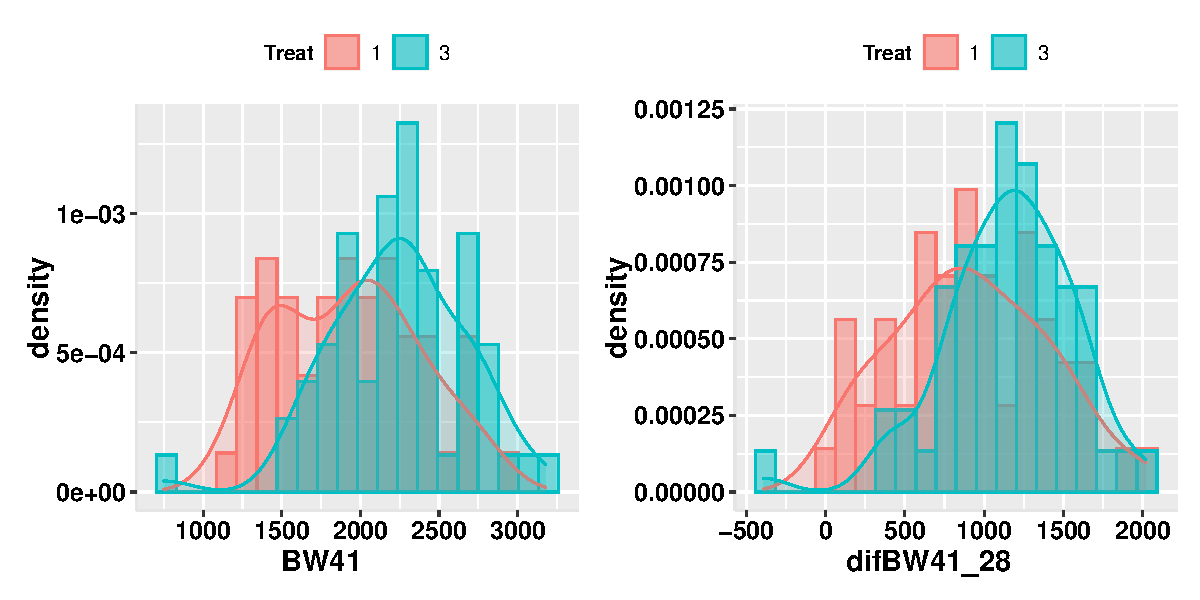
\includegraphics[width=\maxwidth]{figure/unnamed-chunk-9-1} 

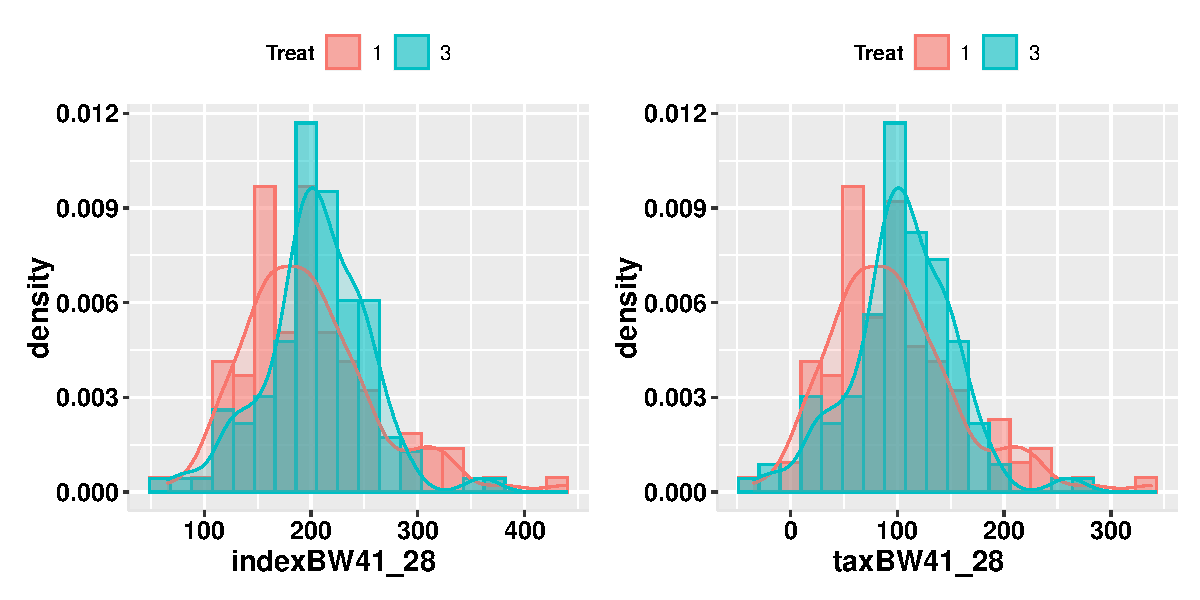
\includegraphics[width=\maxwidth]{figure/unnamed-chunk-9-2} 

\end{knitrout}

\clearpage
\subsection{Comparació de tots els tractaments amb el control}



\subsubsection{Variable \texttt{BW41}}
\begin{knitrout}
\definecolor{shadecolor}{rgb}{0.969, 0.969, 0.969}\color{fgcolor}
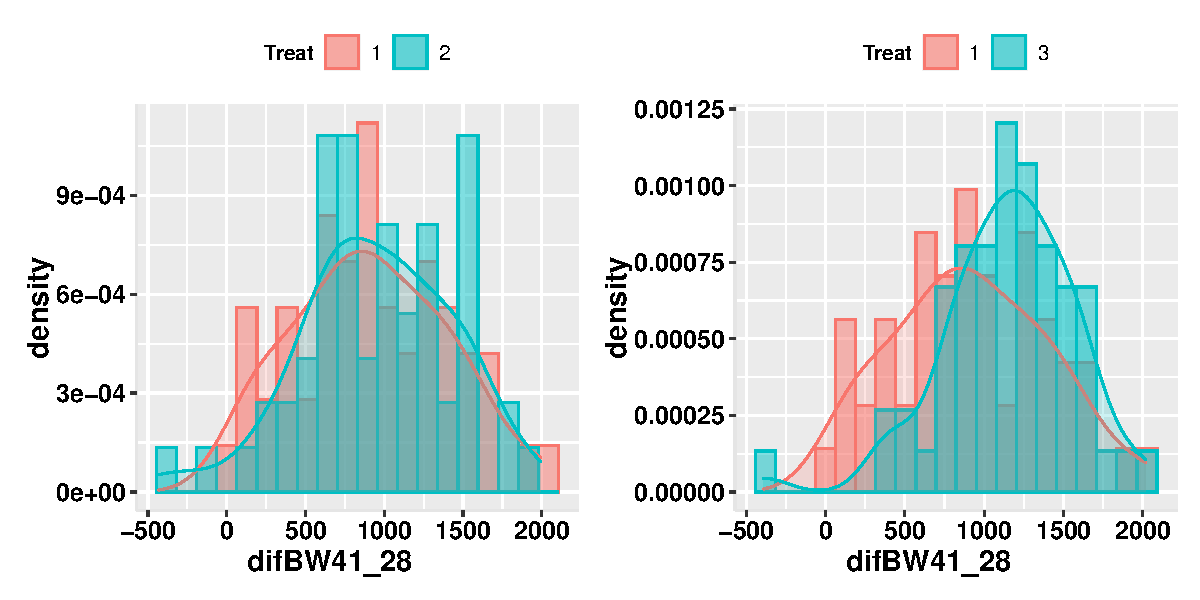
\includegraphics[width=\maxwidth]{figure/unnamed-chunk-11-1} 

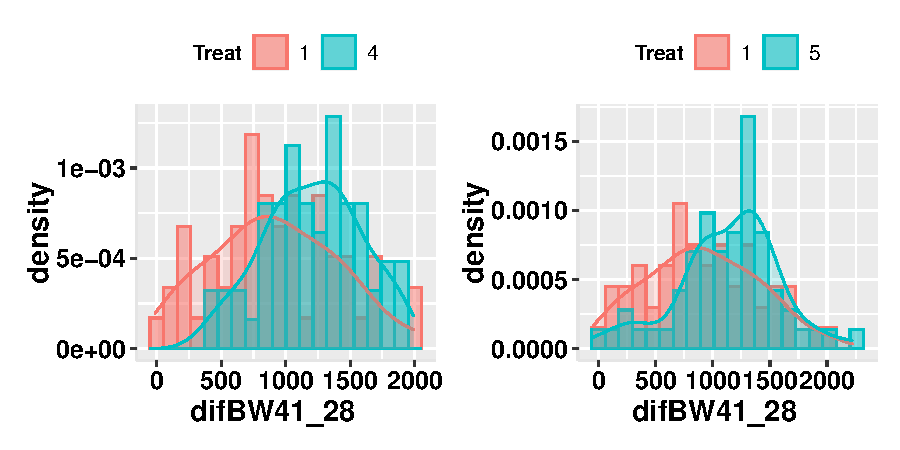
\includegraphics[width=\maxwidth]{figure/unnamed-chunk-11-2} 

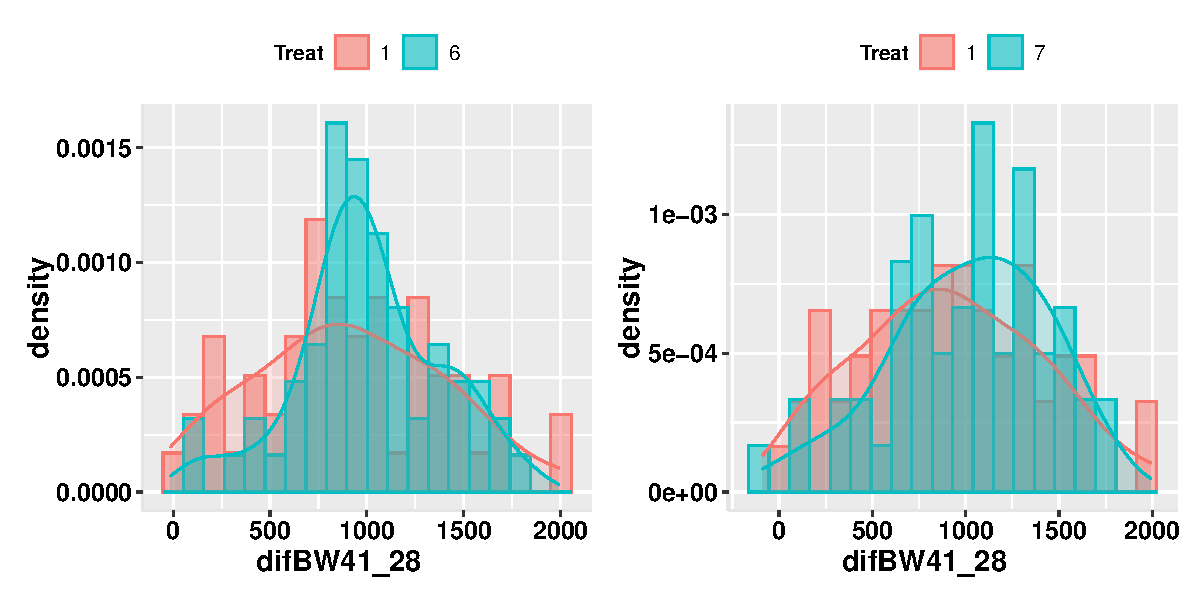
\includegraphics[width=\maxwidth]{figure/unnamed-chunk-11-3} 

\end{knitrout}

\begin{knitrout}
\definecolor{shadecolor}{rgb}{0.969, 0.969, 0.969}\color{fgcolor}
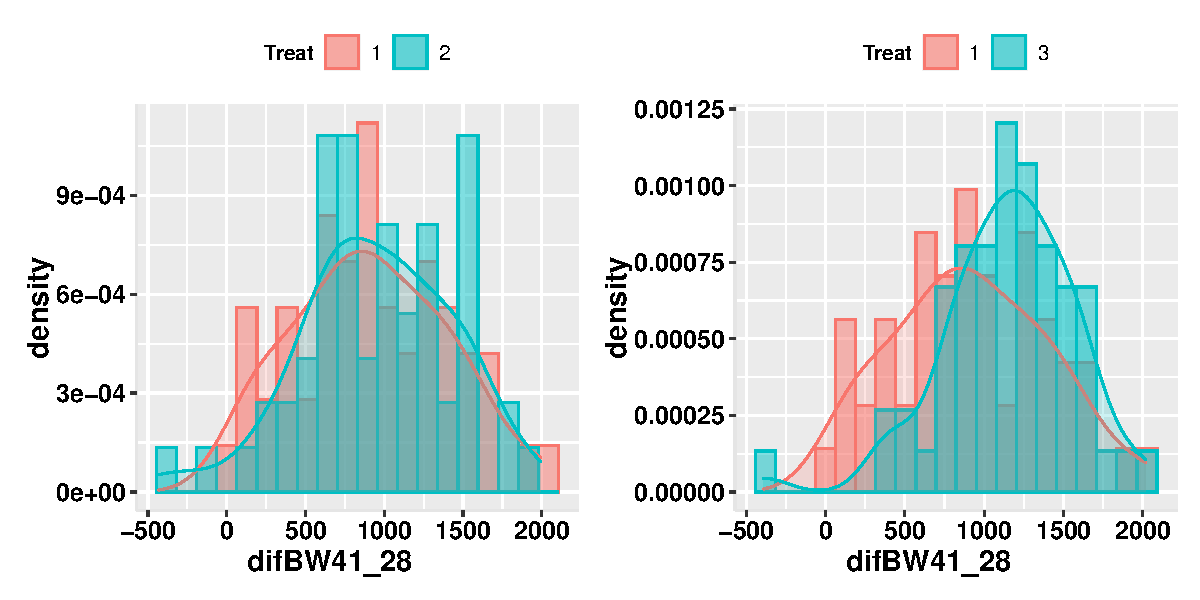
\includegraphics[width=\maxwidth]{figure/unnamed-chunk-12-1} 

\end{knitrout}


\clearpage
\subsubsection{Variable \texttt{difBW$41_{28}$}}

\begin{knitrout}
\definecolor{shadecolor}{rgb}{0.969, 0.969, 0.969}\color{fgcolor}
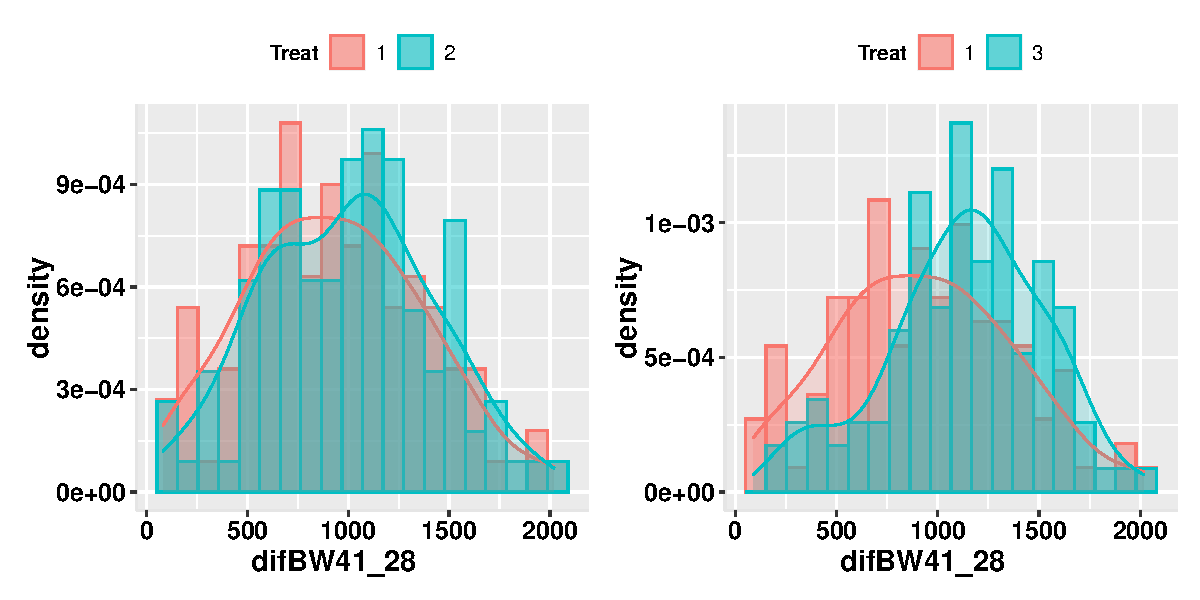
\includegraphics[width=\maxwidth]{figure/unnamed-chunk-13-1} 

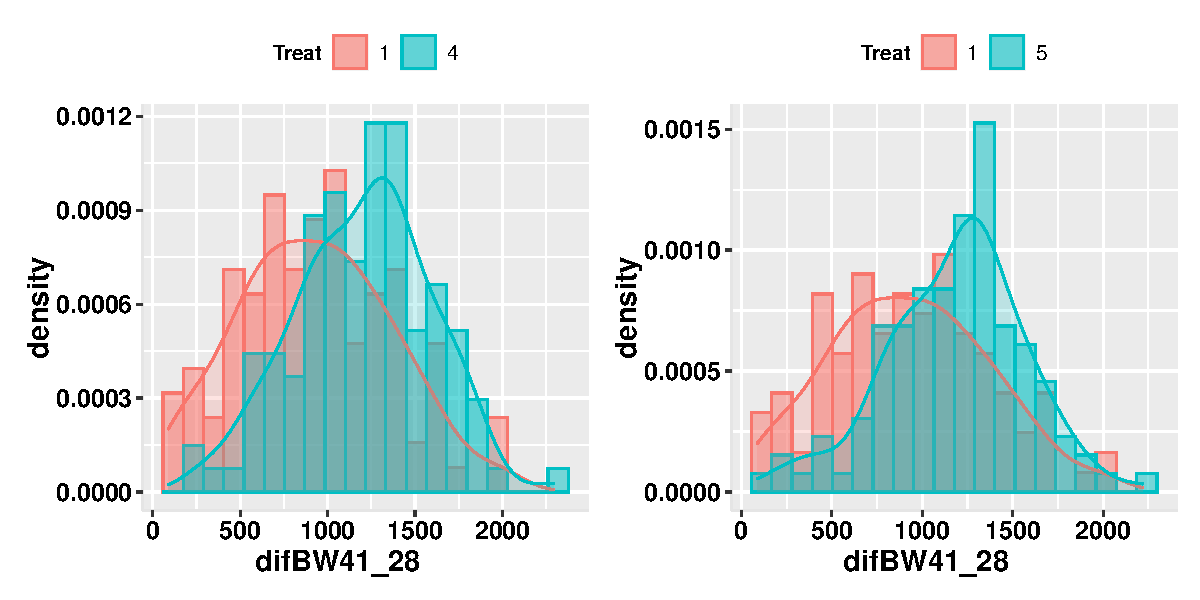
\includegraphics[width=\maxwidth]{figure/unnamed-chunk-13-2} 

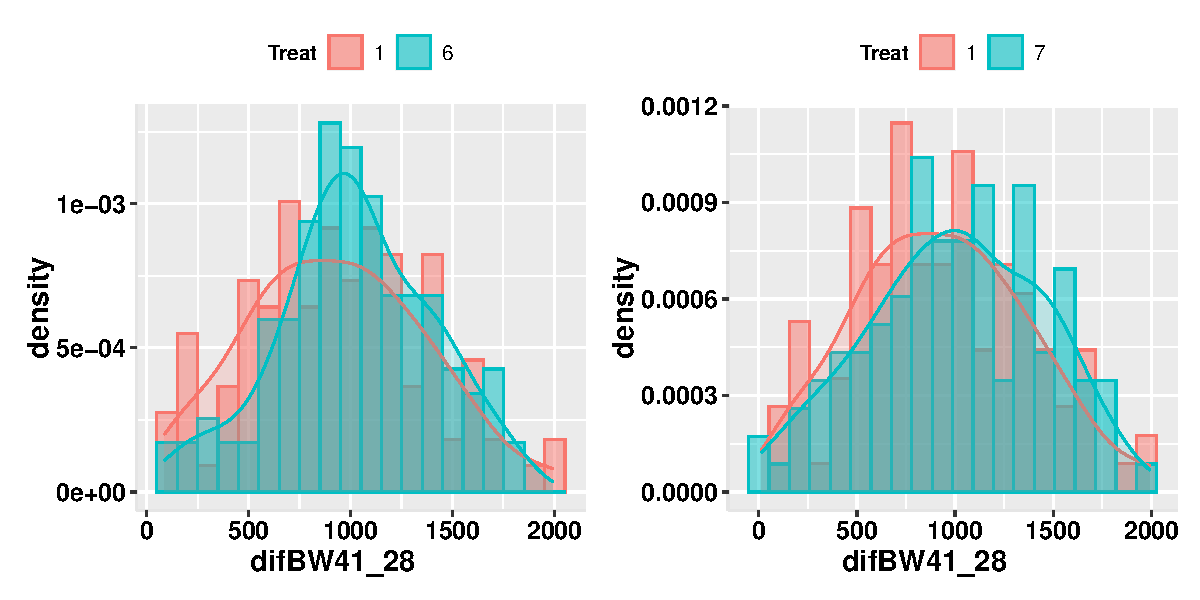
\includegraphics[width=\maxwidth]{figure/unnamed-chunk-13-3} 

\end{knitrout}

\begin{knitrout}
\definecolor{shadecolor}{rgb}{0.969, 0.969, 0.969}\color{fgcolor}
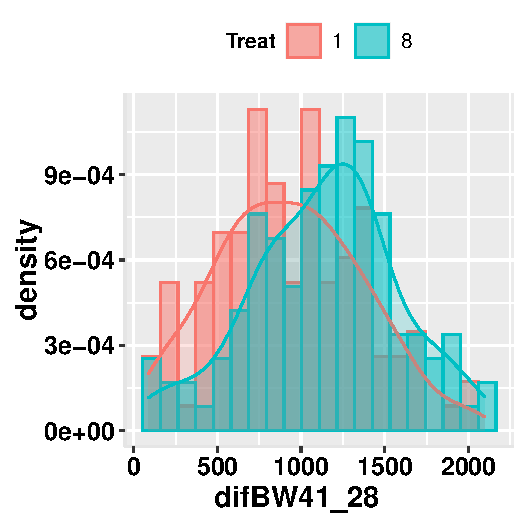
\includegraphics[width=\maxwidth]{figure/unnamed-chunk-14-1} 

\end{knitrout}



\clearpage
\section{Two-Sample Rank Test to detect a shift in a proportion of the ''treated'' population}



Test bi-mostral per detectar un canvi positiu en una proporció de la població (tractament) comparada a una altra (control).

\texttt{quantileTest(x, y, alternative = ''greater'', target.quantile = 0.5, target.r = NULL, exact.p = TRUE)}
    
\begin{itemize}
  \item \texttt{x}: Vector numèric d'observacions del grup tractament.
  
  \item \texttt{y}: Vector numèric d'observacions del grup control.
  
  \item \texttt{alternative}: Tipus d'hipòtesi alternativa.

\begin{itemize}
      \item ''greater'': La cua dreta del grup tractament desplaçada cap a la dreta de la cua dreta del grup control.
      
      \item ''less'': La cua esquerra del grup tractament desplaçada cap a la esquerra de la cua esquerra del grup control.
\end{itemize}


  \item \texttt{target.quantile}: Quantil utilitzat com a punt de tall inferior per a la prova. A causa de la naturalesa discreta dels quantils empírics, el límit superior dels possibles quantils empírics sovint difereix del valor de target.quantile.

\end{itemize}

\textit{$H_1:$ La porció $\epsilon$ de la distribució per al grup de tractament (la distribució de X) es desplaça cap a la dreta de la distribució per al grup de referència (la distribució de Y).}



\subsection{Resultats del test comparant Tractament vs. control}

Apliquem el test al quantil 0.2, 0.3, 0.4 i 0.75. De manera que per exemple per al quantil 0.2 un 20\% de la població és menor o igual al valor del quantil. I a la variable diferència dels pesos individuals a la setmana 28 i a la setmana 41.\\

Veiem un exemple de la sortida de RStudio i una taula resumint els resultats per a a tots els tractaments respecte el control.





\clearpage

% latex table generated in R 3.6.3 by xtable 1.8-4 package
% Tue Dec 29 16:33:35 2020
\begin{table}[ht]
\centering
\begingroup\fontsize{12pt}{12pt}\selectfont
\begin{tabular}{lllllllll}
  \toprule
{\textbf{Treat}} & {\textbf{$q_{20}$}} & {\textbf{P-value}} & {\textbf{$q_{30}$}} & {\textbf{P-value}} & {\textbf{$q_{40}$}} & {\textbf{P-value}} & {\textbf{$q_{75}$}} & {\textbf{P-value}} \\ 
  \midrule
1 & 503 & 0.32064 & 667 & 0.32084 & 772 & 0.26627 & 1221 & 0.26858 \\ 
  2 & 573.8 &  & 693.8 &  & 820.8 &  & 1266.5 &  \\ 
   &  &  &  &  &  &  &  &  \\ 
  1 & 503 & 0.00325 & 667 & 8e-05 & 772 & 0.00064 & 1221 & 0.05803 \\ 
  3 & 819 &  & 936.2 &  & 1060.6 &  & 1381.5 &  \\ 
   &  &  &  &  &  &  &  &  \\ 
  1 & 503 & 4e-05 & 667 & 0 & 772 & 2e-05 & 1221 & 0.00217 \\ 
  4 & 883.6 &  & 1011.6 &  & 1125.4 &  & 1435 &  \\ 
   &  &  &  &  &  &  &  &  \\ 
  1 & 503 & 9e-05 & 667 & 2e-05 & 772 & 3e-05 & 1221 & 0.03003 \\ 
  5 & 865.8 &  & 987.2 &  & 1132 &  & 1419.75 &  \\ 
   &  &  &  &  &  &  &  &  \\ 
  1 & 503 & 0.00555 & 667 & 0.00318 & 772 & 0.02565 & 1221 & 0.24579 \\ 
  6 & 745.2 &  & 849.4 &  & 932.8 &  & 1300 &  \\ 
   &  &  &  &  &  &  &  &  \\ 
  1 & 503 & 0.29542 & 667 & 0.11261 & 772 & 0.1908 & 1221 & 0.06462 \\ 
  7 & 609 &  & 779.7 &  & 865.6 &  & 1357.25 &  \\ 
   &  &  &  &  &  &  &  &  \\ 
  1 & 503 & 0.01499 & 667 & 0.00143 & 772 & 0.0033 & 1221 & 0.03461 \\ 
  8 & 766 &  & 885.5 &  & 1045 &  & 1405 &  \\ 
   &  &  &  &  &  &  &  &  \\ 
   \bottomrule
\end{tabular}
\endgroup
\caption{Taula d'anàlisi de quantiles per a la variable guany de pes $BW41_{28}$} 
\label{tab:tot}
\end{table}



\clearpage
\section{Costos}

Usarem la variable \texttt{Coste\_per PV} del fitxer \texttt{CalculoIndices.xlsx} modificat.\\

La variable s'ha calculat de la següent forma:
$$
\mbox{\text{Cost/kg PV (\EUR{}/kg) = (cost pinso [\EUR{}/kg] * consum pinso [kg]) / guany pes [kg]}}
$$


\vspace{0.5cm}
\subsection{Exploració de la variable Cost}
\begin{knitrout}
\definecolor{shadecolor}{rgb}{0.969, 0.969, 0.969}\color{fgcolor}
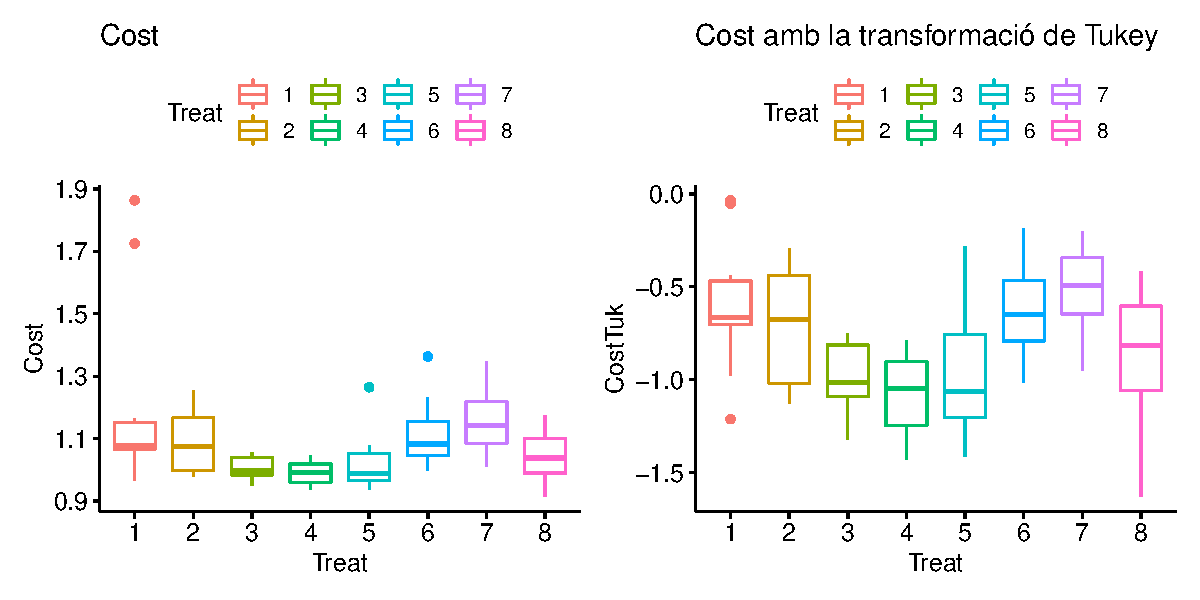
\includegraphics[width=\maxwidth]{figure/unnamed-chunk-20-1} 

\end{knitrout}

Per tal de millorar la normalitat del costos apliquem una transformació de Tukey de la llibreria \texttt{rcompanion}:

{\footnotesize
\begin{knitrout}
\definecolor{shadecolor}{rgb}{0.969, 0.969, 0.969}\color{fgcolor}\begin{kframe}
\begin{verbatim}
## 
##     lambda      W Shapiro.p.value
## 585   -5.4 0.9906          0.8288
## 
## if (lambda >  0){TRANS = x ^ lambda} 
## if (lambda == 0){TRANS = log(x)} 
## if (lambda <  0){TRANS = -1 * x ^ lambda}
\end{verbatim}
\end{kframe}
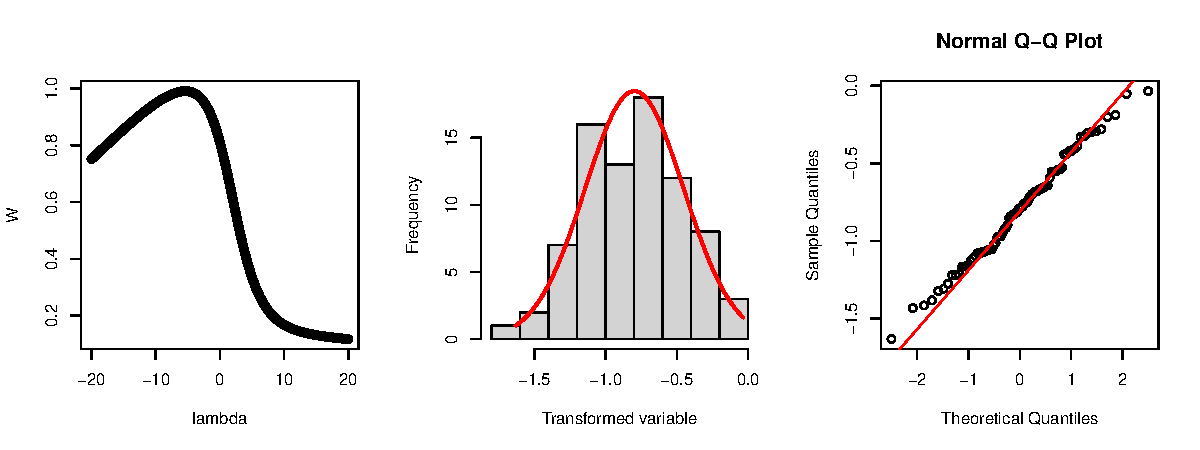
\includegraphics[width=\maxwidth]{figure/unnamed-chunk-21-1} 

\end{knitrout}
}

El programa selecciona una lambda de $-5.4$ de manera que com $\lambda < 0$ la tranformació aplicada als costos serà $costTuk = -1 * Cost^{\lambda}$
\vspace{0.5cm}

\begin{knitrout}
\definecolor{shadecolor}{rgb}{0.969, 0.969, 0.969}\color{fgcolor}
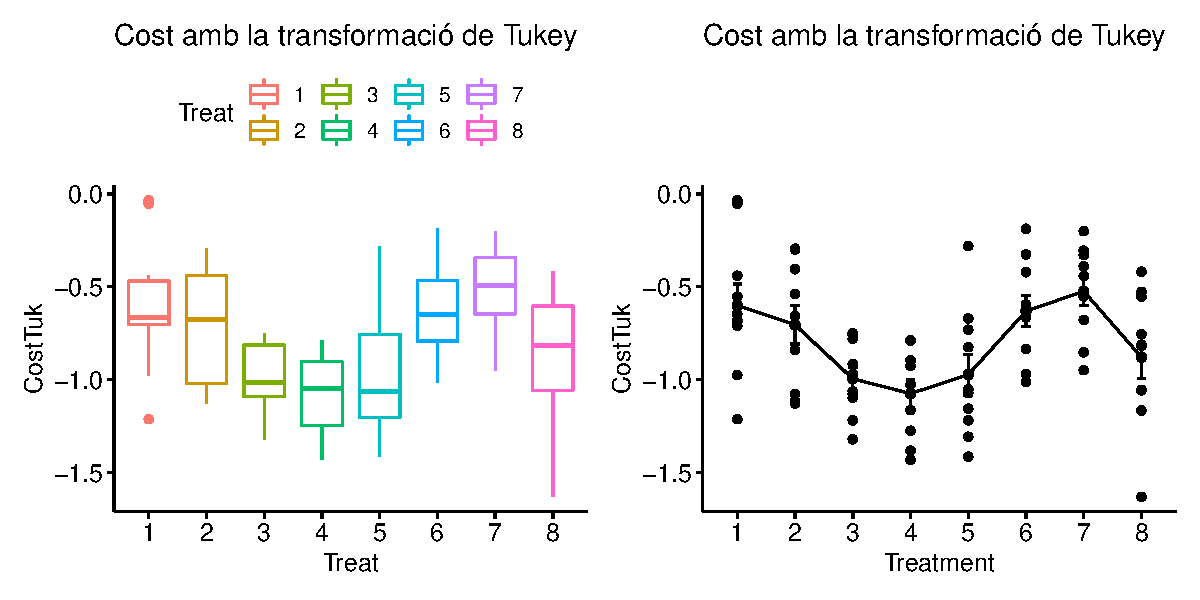
\includegraphics[width=\maxwidth]{figure/unnamed-chunk-22-1} 

\end{knitrout}

\subsection{Anàlisi dels resultats}
Amb les dades normalitzades ajustem un model ANOVA i realitzem els següents tests:

{\footnotesize
\begin{knitrout}
\definecolor{shadecolor}{rgb}{0.969, 0.969, 0.969}\color{fgcolor}\begin{kframe}
\begin{verbatim}
##             Df Sum Sq Mean Sq F value   Pr(>F)    
## Treat        7  3.035  0.4336   4.881 0.000152 ***
## Residuals   72  6.397  0.0888                     
## ---
## Signif. codes:  0 '***' 0.001 '**' 0.01 '*' 0.05 '.' 0.1 ' ' 1
\end{verbatim}
\end{kframe}
\end{knitrout}
}

\paragraph{Tukey multiple pairwise-comparisons:}

Crea un conjunt d'intervals de confiança per les diferències de les mitjanes per als diferents tractaments.

{\footnotesize
\begin{knitrout}
\definecolor{shadecolor}{rgb}{0.969, 0.969, 0.969}\color{fgcolor}\begin{kframe}
\begin{verbatim}
##            diff        lwr         upr      p adj
## 2-1 -0.10534095 -0.5214742  0.31079227 0.99313670
## 3-1 -0.39553259 -0.8116658  0.02060063 0.07431879
## 4-1 -0.47522197 -0.8913552 -0.05908875 0.01427889
## 5-1 -0.37332879 -0.7894620  0.04280442 0.11097158
## 6-1 -0.03179923 -0.4479324  0.38433399 0.99999757
## 7-1  0.07552814 -0.3406051  0.49166136 0.99915669
## 8-1 -0.27980476 -0.6959380  0.13632846 0.42544395
\end{verbatim}
\end{kframe}
\end{knitrout}
}


Si observem el p-valor ajustat per comparacions múltiples observem que els tractments més significatius respecte del control són els tractaments 4,3 i 5, en ordre de significació.

\vspace{0.5cm}
\clearpage
\paragraph{Pairwise t-test:}

Calcula comparacions per parelles entre els diferents tractaments, primer sense i després amb correccions per a proves múltiples. La primera taula conté el p-value usuals del t-test i la de sota conté el p-value ajustat pel mètode de Benjamin  \& Hockberg (BH), un p-valor que ens indica els False Discovery Rate (FDR). Se solen considerar significatives totes les diferències amb un  adj-p-values menor que 0.1.

{\footnotesize
\begin{knitrout}
\definecolor{shadecolor}{rgb}{0.969, 0.969, 0.969}\color{fgcolor}\begin{kframe}
\begin{verbatim}
## 
## 	Pairwise comparisons using t tests with pooled SD 
## 
## data:  costos$CostTuk and costos$Treat 
## 
##   1       2       3       4       5       6       7      
## 2 0.43197 -       -       -       -       -       -      
## 3 0.00408 0.03276 -       -       -       -       -      
## 4 0.00065 0.00703 0.55183 -       -       -       -      
## 5 0.00654 0.04813 0.86817 0.44713 -       -       -      
## 6 0.81213 0.58286 0.00798 0.00139 0.01250 -       -      
## 7 0.57274 0.17906 0.00072 9.6e-05 0.00122 0.42338 -      
## 8 0.03932 0.19476 0.38818 0.14700 0.48518 0.06690 0.00948
## 
## P value adjustment method: none
## 
## 	Pairwise comparisons using t tests with pooled SD 
## 
## data:  costos$CostTuk and costos$Treat 
## 
##   1      2      3      4      5      6      7     
## 2 0.5691 -      -      -      -      -      -     
## 3 0.0190 0.0764 -      -      -      -      -     
## 4 0.0067 0.0246 0.6277 -      -      -      -     
## 5 0.0246 0.0963 0.8682 0.5691 -      -      -     
## 6 0.8422 0.6277 0.0248 0.0078 0.0318 -      -     
## 7 0.6277 0.2949 0.0067 0.0027 0.0078 0.5691 -     
## 8 0.0847 0.3030 0.5691 0.2572 0.5907 0.1249 0.0265
## 
## P value adjustment method: BH
\end{verbatim}
\end{kframe}
\end{knitrout}
}

Observem les comparacions per parelles de tractaments sense cap tipus de correcció (p-valors més petits) i amb la correcció de Benjamin \& Hochberg que controla el rati de falsos positius a l'hora de fer múltiples comparacions.\\

Cal destacar que les diferències en els p-valors per a les comparacions dos a dos es deuen a que el t.test i les comparacions de Tukey utilitzen metodologies diferents per a obtenir el p-valor.\\

Els resultats de la correcció de Tukey i de BH no coincideixen perquè la correcció de Tukey és més conservadora. Ens inclinem per presentar aquesta segona opció: p-value sense ajustar i ajustat per BH.


\clearpage

%%%%%%%%%%%%%%%
%%%
%%% References
%%%
%%%%%%%%%%%%%%%
\begin{thebibliography}{x}

\bibitem{ggplot2}
\url{https://www.rdocumentation.org/packages/ggplot2/versions/3.3.2}

\bibitem{devtools}
\url{https://www.rdocumentation.org/packages/devtools/versions/2.3.2}

\bibitem{easyGgplot2}
\url{https://github.com/kassambara/easyGgplot2}

\bibitem{patchwork}
\url{https://www.rdocumentation.org/packages/patchwork/versions/1.1.0}

\bibitem{EnvStats}
\url{https://www.rdocumentation.org/packages/EnvStats/versions/2.4.0}

\bibitem{quantileTest}
\url{https://www.rdocumentation.org/packages/EnvStats/versions/2.3.1/topics/quantileTest}\\
\url{https://www.jstor.org/stable/2532001?seq=1&cid=pdf-reference}

\bibitem{xtable}
\url{https://www.rdocumentation.org/packages/xtable/versions/1.8-4}

\bibitem{rcompanion}
\url{https://www.rdocumentation.org/packages/rcompanion/versions/2.3.26}

\bibitem{ggpubr}
\url{https://www.rdocumentation.org/packages/ggpubr/versions/0.4.0}

\bibitem{aov}
\url{https://www.rdocumentation.org/packages/stats/versions/3.6.2/topics/aov}

\bibitem{TukeyHSD}
\url{https://www.rdocumentation.org/packages/stats/versions/3.6.2/topics/TukeyHSD}

\bibitem{pairwise.t.test}
\url{https://www.rdocumentation.org/packages/stats/versions/3.6.2/topics/pairwise.t.test}

\bibitem{levene.test}
\url{https://www.rdocumentation.org/packages/lawstat/versions/3.2/topics/levene.test}


\end{thebibliography}



\end{document}
